\RequirePackage[T1]{fontenc}
\documentclass[conference,letterpaper]{IEEEtran}

\usepackage{cite}
\usepackage{amsmath,amssymb}
\usepackage{graphicx}
\usepackage{booktabs}
\usepackage{array}
\usepackage{xurl}
\usepackage[hidelinks]{hyperref}
\hypersetup{
  pdftitle={Counterfactual Shadow Continuum: Non-Actuating Shadow Execution for Cloud--Edge Decision Evaluation},
  pdfauthor={Uma Patil; Adish Nair; Sumit Mane; Nihar Mehakare; Apurva Mendgule},
  pdfsubject={Controlled shadow execution and simulation-referenced evaluation},
  pdfkeywords={shadow execution, counterfactual evaluation, SUMO, reproducibility}
}

\makeatletter
\newcommand{\linebreakand}{%
  \end{@IEEEauthorhalign}
  \hfill\mbox{}\par
  \mbox{}\hfill\begin{@IEEEauthorhalign}
}
\makeatother

\begin{document}

\title{Counterfactual Shadow Continuum: Non-Actuating Shadow Execution for Cloud--Edge Decision Evaluation}

\author{
\IEEEauthorblockN{Dr. Uma Patil}
\IEEEauthorblockA{
\textit{Department of CSE(AIML)}\\
\textit{Vishwakarma Institute of Technology}\\
Pune, India\\
uma.patil@vit.edu
}
\and
\IEEEauthorblockN{Adish Nair}
\IEEEauthorblockA{
\textit{Department of CSE(AIML)}\\
\textit{Vishwakarma Institute of Technology}\\
Pune, India\\
adish.nair24@vit.edu
}
\and
\IEEEauthorblockN{Sumit Mane}
\IEEEauthorblockA{
\textit{Department of CSE(AIML)}\\
\textit{Vishwakarma Institute of Technology}\\
Pune, India\\
sumit.mane24@vit.edu
}

\linebreakand

\IEEEauthorblockN{Nihar Mehakare}
\IEEEauthorblockA{
\textit{Department of CSE(AIML)}\\
\textit{Vishwakarma Institute of Technology}\\
Pune, India\\
nihar.mehakare24@vit.edu
}
\and
\IEEEauthorblockN{Apurva Mendgule}
\IEEEauthorblockA{
\textit{Department of CSE(AIML)}\\
\textit{Vishwakarma Institute of Technology}\\
Pune, India\\
apurva.mendgule24@vit.edu
}
}

\maketitle

\begin{abstract}
Decision systems observe chosen actions while alternatives remain unobserved.
Counterfactual Shadow Continuum (CSC) separates authoritative production from a
same-action mirror and non-actuating alternative branches. State anchors and
bounded evidence admission support comparison without transferring actuation
authority. We evaluated runtime behavior, Kubernetes containment and
forecast-only estimates against Simulation of Urban MObility (SUMO), all on one
physical host. Across 864 execution configurations and six seed clusters,
alternative queue mean absolute error was 2.029 vehicles versus 3.841 for a
stationary persistence baseline, a 47.18\% reduction. Best-action agreement was
0.778 (77.78\%), versus 0.222 for persistence. The predictor uses arrival
forecasts and calibration; the baseline ignores both, so this accuracy difference
is not an effect of branching or mirrors. An infrastructure pilot completed 120
requests. Complete evidence collapsed under added shadow delay, the continuous
study was not executed, and memory containment remained inconclusive after the
observer was killed. These results demonstrate bounded execution and simulator
comparisons. Limited replication, incomplete containment and the absence of
physical counterfactual observations restrict their use for operational decisions;
learning and policy promotion remain blocked.
\end{abstract}

\begin{IEEEkeywords}
shadow execution, counterfactual evaluation, evidence admission, fault containment,
traffic simulation, Kubernetes
\end{IEEEkeywords}

\section{Introduction}
A controller observes the trajectory produced by its chosen action, while the
outcomes of alternatives remain missing. This selective-feedback problem
motivates counterfactual and off-policy evaluation
\cite{bottou2013counterfactual,li2011unbiased,wang2017optimal}. Online exploration
can provide information but exposes production to unvalidated behavior. Digital
twins offer virtual representations for comparison, subject to modeling,
synchronization and validation challenges \cite{tao2019digital,fuller2020digital}.

Counterfactual Shadow Continuum (CSC) asks a systems question: can alternative
branches execute from a captured decision state without production authority,
and can incomplete, late or invalid evidence be excluded from comparison?
The architecture targets cloud--edge decision systems, but every experiment
reported here ran on one physical host; Kubernetes nodes were logical nodes.
Production outcomes are factual only within the declared software environment.
Alternative simulator trajectories are simulation-based references, not observed
physical causal counterfactuals. CSC collects evidence; it does not identify
causal effects or authorize a learned policy.

The contributions are:
\begin{itemize}
\item An implemented separation of the production branch, a same-action mirror
and distinct alternative branches, with state anchors, bounded admission and
reusable workers.
\item An evaluation of evidence completeness, execution cost and selected
containment controls, including delay collapse, incomplete resource enforcement
and an unexecuted continuous study.
\item An independent-simulator evaluation of forecast-only fluid estimates,
with paired execution modes, calibration separated from evaluation, and
condition-specific negative findings.
\end{itemize}
The prediction comparison is deliberately limited: a calibrated fluid predictor
uses past-arrival forecasts, while a stationary persistence baseline ignores
forecasts and calibration. Its error reduction measures that predictor comparison.
CSC's measured architectural effects concern evidence completeness, containment
and execution cost.

We ask: (RQ1) does the development-calibrated, forecast-using predictor reduce
alternative queue error relative to persistence; (RQ2) how do action agreement, simulation-derived regret
and mirror error vary with horizon and model mismatch; and (RQ3) do execution
modes preserve the production trajectory, and at what execution cost?

\section{Related Work}
Digital twins link virtual representations with physical assets, but model
fidelity and synchronization remain central challenges
\cite{tao2019digital,fuller2020digital}. Production traffic mirroring already
copies requests outside the primary response path \cite{istio-mirroring}.
CSC adds alternative-action execution from a captured state and explicit
admission of comparison evidence. The validity of those alternatives still
depends on the model.

Counterfactual and off-policy methods estimate outcomes or policy value from
logged interventions \cite{bottou2013counterfactual}. Randomized logging and
action matching can support unbiased replay \cite{li2011unbiased}; doubly robust
and adaptive estimators address model error and statistical overlap
\cite{jiang2016doubly,wang2017optimal}. CSC instead executes a transition model
from captured state and declared inputs. It requires model fidelity,
synchronization and timely completion rather than inheriting an unbiased
policy-value guarantee. Safe reinforcement learning constrains exploration or
policy optimization \cite{garcia2015safe,achiam2017cpo}; CSC operates before
that stage by retaining non-actuation and excluding unsuitable evidence.

Cloud--edge research motivates placement near data sources
\cite{shi2016edge,satyanarayanan2017edge}. Dependability research distinguishes
faults, failures and containment mechanisms \cite{avizienis2004dependable}, while
lightweight virtualization offers stronger isolation options
\cite{agache2020firecracker}. CSC evaluates selected Kubernetes controls instead
\cite{k8s-networkpolicy,k8s-securitycontext,k8s-resources,k8s-images}.
Simulation of Urban MObility (SUMO) provides independently implemented microscopic dynamics and a Traffic
Control Interface (TraCI) \cite{sumo2018}. Distributed speculative execution,
including MapReduce, addresses redundant work and variable completion times
\cite{dean2004mapreduce}. CSC's alternative branches compare different decisions,
so redundant execution alone cannot establish their predictive validity.

Table~\ref{tab:literature-positioning} locates the contribution: a concrete
execution and evidence-admission architecture, evaluated across these boundaries.
The comparison does not establish unique novelty or remove the assumptions
needed for causal inference.
\begin{table*}[t]
\caption{Positioning Relative to Adjacent Literature}
\label{tab:literature-positioning}
\centering
\begin{tabular}{@{}>{\raggedright\arraybackslash}p{0.18\textwidth}>{\raggedright\arraybackslash}p{0.32\textwidth}>{\raggedright\arraybackslash}p{0.45\textwidth}@{}}
\toprule
Area & Established focus & CSC's scope and remaining gap \\
\midrule
Digital twins & Physical--virtual representation and synchronization & Same-action comparison; physical fidelity remains unvalidated. \\
Off-policy evaluation & Statistical estimation from logged interventions & Model-execution evidence, without an unbiased policy-value guarantee. \\
Safe learning & Optimization under constraints & Evidence admission before learning; no policy optimization or certification. \\
Cloud--edge computing & Placement and distributed execution & Delay and execution-cost measurements on one physical host. \\
Dependability & Fault containment and failure handling & Selected Kubernetes controls, without whole-host containment. \\
\bottomrule
\end{tabular}
\end{table*}

\section{Problem Formulation}
At epoch $t$, a coordinator captures a state anchor $s_t$ and an ordered input
window $x_t$. An anchor is a serialized state snapshot with a content hash and
observation watermark. The production branch chooses $a_t^p$ and alone may
mutate the authoritative environment. A mirror executes that same action in a
model. The $K$ alternative branches execute distinct admissible actions
$a\ne a_t^p$; $K$ excludes the mirror.

Complete evidence means that the mirror and every requested alternative
completed with valid state, input and branch provenance. Missing or invalid
outcomes are excluded rather than imputed. For utilities $U_t^p$ and $U_t^m$
over the production and mirror windows, the post-window discrepancy is
\begin{equation}
 \epsilon_t=|U_t^p-U_t^m|.
 \label{eq:mirror-gap}
\end{equation}
Utility is negative mean total queue in the traffic domain. The mirror
queue error reported below is the queue-domain form of this absolute gap.
The gap becomes available during or after the window; it is a retrospective
diagnostic, not a validated pre-decision safety signal. Offline replay may use
a recorded input window. Online prediction, in contrast, receives only
observations available at its decision watermark.

\section{CSC Architecture}
Figure~\ref{fig:architecture} shows the authority boundary. The coordinator owns
state capture, branch assignment and evidence admission. A production request
passes through a token gateway before reaching the authoritative environment.
Mirror and alternative workers receive state, actions and inputs without
production signing material. Their virtual actuator boundary (VAB) records
requested actions locally without forwarding them to production.

Cold workers start a process for each branch. Warm workers reset and rehydrate
before reuse, validate the anchor and fresh input buffers, reset random state,
and enforce reuse limits. In asynchronous mode, production commits without
waiting for shadows. A bounded ledger tracks outstanding work, expiry,
duplicates and comparison completion. This removes a logical dependency while
retaining shared processor, memory, storage and input/output resources.

Evidence admission checks branch provenance, state and input hashes, schemas,
completion and deadlines. It is fail-closed in the specific sense that invalid
or incomplete branches are not admitted as complete evidence. Append-only
archives retain research records. A bounded spool supports best-effort optional
evidence persistence. The trust decision remains separate from completion;
learning and policy promotion are blocked.

The deployment was later extended with Redis assignment authorization and NATS
result transport. Only the coordinator writes Redis assignments, using
create-if-absent writes and a 180-s time to live (TTL). Worker access control
lists (ACLs) permit reads only from the worker's own assignment keys and deny
access to protected epoch records. NATS authenticates roles and restricts each
worker to its own publication subject. Workers cannot subscribe; the coordinator
subscribes to results but cannot publish. The receiver verifies a per-worker
hash-based message authentication code (HMAC), experiment and epoch binding,
branch and subject, role, action, state and input hashes, schema and replay
status. Admitted messages remain estimates and carry no actuation authority.

\begin{figure*}[t]
\centering
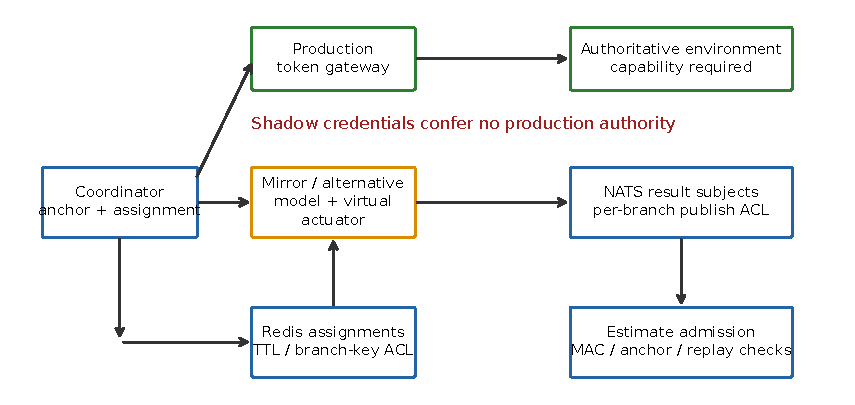
\includegraphics[width=0.96\textwidth]{figures/architecture.pdf}
\caption{Implemented authority and evidence paths. Redis assigns work and NATS
transports estimates; production retains the token gateway. ACL denotes access
control list, TTL time to live, and MAC message authentication code. This is an
architecture diagram, not a measurement or confidence interval.}
\label{fig:architecture}
\end{figure*}

\section{Prototype and Implementation}
The reference traffic domain has one intersection and three actions:
\texttt{NS\_GREEN} serves north--south approaches, \texttt{EW\_GREEN} serves
east--west approaches, and \texttt{BALANCED} divides the window between them.
In the runtime experiment, independent production and fluid-model transitions
use the same declared state and inputs. Content hashes identify serialized anchors. HMAC-bound tokens carry
role, branch, action, epoch, expiration and experiment. The gateway validates
these claims and uses a lock-protected one-plan-per-epoch interlock.
Synchronization checks sequence, duplicates and input hashes.

Kubernetes separates environment, gateway, coordinator and workers. Controls
include network policies, non-root execution, read-only root filesystems,
disabled privilege escalation, dropped capabilities, no host mounts,
resource requests and limits, and explicit placement
\cite{k8s-networkpolicy,k8s-securitycontext,k8s-resources}. Exact container images
were preloaded on all three logical nodes and used without registry pulls
\cite{k8s-images}. The authorization services used Redis 7.4.2 and NATS 2.10.26,
with client versions 5.2.1 and 2.9.0, respectively. Their permission mechanisms
are documented by the projects \cite{redis-acl,nats-authorization}.
Ephemeral Kubernetes Secrets supply separate coordinator and worker credentials.
Workers receive no production signing or environment key, and broker
configuration is not mounted in their containers.

The simulator study used Windows 11 build 26300, Python 3.14.7, an Intel Core 5
210H with 8 cores and 12 logical processors, and 16,788,983,808 bytes of random
access memory. SUMO, TraCI and associated packages were pinned to 1.28.0.
Only a capability-bound production component holds the live TraCI connection;
predictors receive an aggregate anchor, action, horizon and model rate.
The simulator evaluation uses threads, whereas the runtime study uses process
workers. Their timing measurements describe different execution configurations.

\section{Experimental Methodology}
We organize the evaluation into E1, runtime evidence yield and fault isolation;
E2, containment and authorization; and E3, independent-simulator evaluation.
Each used a pre-registered protocol with separate development and measurement
artifacts. Configuration, software versions, seeds, raw records, failures and
checksums were preserved. Experimental units and timing scopes differ as
specified below.

\subsection{E1: Runtime Evidence Yield and Fault Isolation}
E1 scheduled 70 runs: 54 factorial runs, 15 optional-storage-fault runs and one
10,000-epoch continuous condition. Factorial comparisons used three paired
450-epoch measured cohorts per configuration. Conditions varied worker reuse,
requested alternatives, added assignment delay, worker capacity and bounded
central processing unit (CPU), memory and storage pressure. Production pacing
was 40 ms. The evidence deadline was 0.3 s after production commit, distinct
from the 2.0-s worker timeout. Late outcomes were excluded from complete
comparisons. Delay results therefore depend on this admission policy, worker
capacity and shared-host scheduling.

Archives were checked for configuration and content hashes, coverage, paired
production and inputs, deterministic replay and authoritative mutations.
The storage experiment separated production survival from generated, spooled,
dropped and durably persisted evidence. The continuous condition required
2 gibibytes (GiB) available memory before starting.

\subsection{E2: Containment and Authorization Evaluation}
E2 tested non-actuation, token authorization, the single-actuation interlock,
network access, filesystem/capability restrictions and resource limits.
Outcomes were PASS, FAIL, INCONCLUSIVE, NOT TESTED or not applicable (N/A).
Configuration alone did not count as observed enforcement. Table~\ref{tab:containment}
retains both initial and revised-test outcomes where the setup changed.
The initial deployment had five matching container images on three ready nodes.
The extended deployment ran seven application/broker pods.

Valid production tokens were bound to the gateway's experiment. One epoch
tested sequential duplicates; another submitted eight independently signed
concurrent requests. The required outcome was one authoritative plan per epoch
and explicit duplicate-denial audit events. Two workers read their Redis
assignments, ran six fluid-model ticks through the VAB, and published results.
Probes attempted protected and cross-branch Redis operations, unauthorized NATS
publication/subscription, and replayed, forged, stale, cross-branch and malformed
results.

For CPU enforcement, a co-located shadow ran one intensive thread for eight
seconds under a 0.25-core quota. Thirty normal and thirty pressure-condition
production plan commits used the same alternating action schedule. Hypertext
Transfer Protocol (HTTP) request latency excluded epoch opening. Control-group
(cgroup) usage and throttling counters bracketed pressure. The comparison was
one normal-then-pressure deployment, not independent request-level replication.
Domain Name System (DNS) resolution and prohibited Transmission Control
Protocol (TCP) contacts had separate reachable positive controls.
A bounded memory probe requested 160 mebibytes (MiB) in a disposable 128-MiB container.
Its criterion required observer survival and an increased out-of-memory (OOM)
counter. The shared process-identifier (PID) allowance was not exhausted.

\subsubsection{Infrastructure service pilot}
A separate infrastructure application programming interface (API) performed CPU
work under replica-count configurations. All branches received identical
requests. This evaluated service execution, image consistency, tested network
boundaries and cleanup. Replica-count alternatives are infrastructure
configurations, distinct from traffic-control actions.

\subsection{E3: Independent-Simulator Evaluation}
\label{sec:sumo-method}
E3 used SUMO's independently implemented microscopic dynamics and TraCI
\cite{sumo2018,sumo-save-state,sumo-tls}. The network had four straight
approaches, one lane each, 200-m incoming roads, 13.89-m/s speed limits and
one-second steps. Signal changes required three seconds of yellow and one
second of all-red, with five seconds minimum green. The balanced action
targeted north--south green in the first half and east--west green in the
second. Unlike the simplified queue model's instantaneous switches, these
operations use explicit intergreens. Turning, pedestrians and lane changes
were excluded.

Five 20-second alternating warmup blocks ended at simulator time 100 s with
stable north--south green. Anchors contained halted queues, phase and age,
past-20-second actual insertion rates, observed lane limits and a watermark.
Predictors used constant past-rate forecasts. They did not receive microscopic
positions, speeds, future departures or saved simulator states. Lane restrictions
were recorded but omitted from the fluid dynamics. A trusted offline evaluator
restored the same microscopic state, demand and random-number-generator state
in a separate process for each of the three actions. Each rollout fully
reloaded the network, routes and saved state; a persistent six-phase signal
program and live link/readback checks rejected invalid control. Collision and
teleport checks were part of validity screening \cite{sumo-save-state}.
Realized future demand was used for reference evaluation only.

Development used two disjoint seeds with moderate/asymmetric demand and 20/40-s
horizons. It selected 1.2 vehicle/s from 0.5, 0.8 and 1.2 vehicle/s by minimum
queue mean absolute error (MAE). Six new evaluation seeds were crossed with
six conditions, two horizons and fixed/queue-responsive production policies.
Conditions were low, moderate and high balanced demand, directional asymmetry,
an unannounced demand increase and a reduced-speed east approach. Planned
Bernoulli departures and actual insertions were recorded separately.

Each of 144 policy/horizon windows evaluated six modes: production only, one
alternative shadow, mirror only, alternatives without a mirror, and a mirror
plus $K=2$ alternatives with synchronous or asynchronous dispatch. Modes shared
initial state, demand, production action and horizon. Their different prediction
counts are reported explicitly. A 1.5-times service-rate ablation changed
predictions only. The stationary persistence baseline predicted the observed
initial queue for every action. It received the same anchor but ignored arrival
forecasts and calibration. Incomplete action sets were excluded from ranking.

For window $i$, action $a$ and horizon $H$, let $q_{i,a,h}^{S}$ be the simulated
total halted queue at step $h$. Its mean is
$q_{i,a}^{S}=H^{-1}\sum_{h=1}^{H}q_{i,a,h}^{S}$, in vehicles.
Let $\widehat q_{i,a}$ be its model prediction and $a_i^p$ the production action.
The per-window alternative error is
\begin{equation}
 e_i^{\mathrm{alt}}=\frac{1}{K}\sum_{a\ne a_i^p}
 |\widehat q_{i,a}-q_{i,a}^{S}|,\qquad K=2.
 \label{eq:alternative-error}
\end{equation}
The reported MAE averages these errors within each seed and then across seeds.
Mirror error is $|\widehat q_{i,a_i^p}-q_{i,a_i^p}^{S}|$.
With predicted-best action $\widehat a_i=\arg\min_a\widehat q_{i,a}$,
simulation-derived regret is
\begin{equation}
 r_i^{S}=q_{i,\widehat a_i}^{S}-\min_a q_{i,a}^{S}
 \quad\text{(vehicles)}.
 \label{eq:simulator-regret}
\end{equation}
This regret uses reference outcomes, not a model-estimated improvement.
Agreement means $\widehat a_i$ belongs to the reference optimum set with
$10^{-9}$ tolerance and a fixed action-order tie break.

TraCI provided queue, lane and vehicle observations \cite{sumo-lanes}.
Stopped-queue integration measures waiting vehicle-seconds. Incoming-lane
exits and completed trips are separate throughput counts. Delay integrates
$\max(0,1-v/v_{\mathrm{allowed}})$ per incoming vehicle per second, where $v$
is observed speed and $v_{\mathrm{allowed}}$ its allowed speed. Only queue
predictions were scored; fluid-model and simulator delay/throughput metrics
were not equated.

The independent resampling unit was the seed ($n=6$), after averaging paired
conditions within each seed. Deterministic 2,000-resample whole-seed percentile
intervals were retained unchanged. The pre-registered RQ1 criterion required
at least 20\% lower mean alternative MAE than persistence and a positive lower
95\% paired interval for the absolute reduction. Mode order was deterministically
permuted within windows. Policy computation, action commitment, total window
wall time, evidence counts and failures were recorded separately. This was a
one-decision-window experiment, not sustained closed-loop control.

\paragraph{Artifact and reproducibility}
A companion artifact index, \path{ARTIFACTS.md}, identifies the archived
protocols, exact source snapshots, image and simulator checksums, seeds, raw
records, analysis exports and reproduction commands. It distinguishes runtime,
containment, service-pilot and simulator datasets. New analysis/build outputs
use unique directories; measured archives are not overwritten. No public
repository, artifact identifier or author approval is asserted here.

\section{Results}
\subsection{E1: Runtime Evidence Yield and Fault Isolation}
E1 executed 69 short runs. The continuous study was NOT TESTED: available memory
was 1,812,451,328 bytes, below the 2-GiB start requirement, so no production
epoch ran. Verification replayed 65,207 branches with zero mismatches and covered
30,000 production epochs. Paired production and input hashes matched, and no
unauthorized authoritative mutation was found.

Table~\ref{tab:runtime} reports the short-run evidence yield and cadence.
Warm $K=2$ completeness remained below full coverage under normal load and
bounded CPU, memory and storage pressure.
Archived execution records include scheduler-capacity drops and failed branch
completions; these prevent completeness from reaching full coverage. The
inspected failure entries do not assign a cause to every failed completion.
The executor reached its 12-task limit and a 43,268-byte serialized-request
high-water mark without executor item or byte rejection. Scheduler admission
drops are distinct from those executor rejection counters.

\begin{table}[t]
\caption{Short-Run Runtime Outcomes. Completeness Uses Cell Medians From Three Paired Runs.}
\label{tab:runtime}
\centering
\begin{tabular}{lr}
\toprule
Measure & Result \\
\midrule
Scheduled / executed / blocked & 70 / 69 / 1 \\
Replays / mismatches & 65,207 / 0 \\
Normal warm $K=2$ completeness & 96.22\% \\
CPU / memory / storage & 95.78 / 96.00 / 93.11\% \\
Worst inter-epoch interval & 61.757 ms \\
Unauthorized mutations & 0 \\
\bottomrule
\end{tabular}
\end{table}

Under the 0.3-s evidence deadline, median complete $K=2$ evidence fell to
0.22\% at 120 ms added delay per assignment and to zero at 400 ms
(Fig.~\ref{fig:delay}). These observations depend on the configured deadline
and admission capacity. With one worker slot, complete requested sets were zero
while 96.44\% of mirrors remained available.
\begin{figure}[t]
\centering
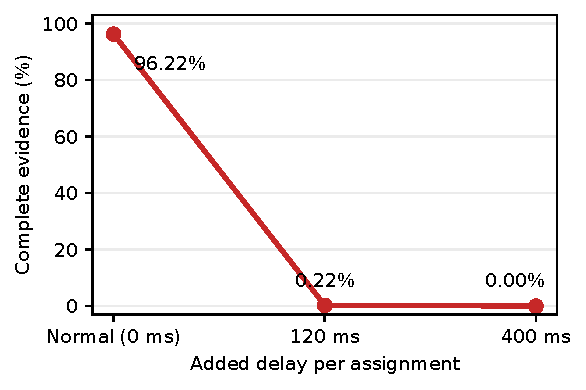
\includegraphics[width=\columnwidth]{figures/evidence_delay.pdf}
\caption{Median complete evidence at the observed delay settings, with three
run units per condition. Lines connect discrete settings; no fitted response or
uncertainty interval is shown. The evidence deadline was 0.3 s after commit.}
\label{fig:delay}
\end{figure}

All 15 optional-store runs retained 200 production epochs. Control,
preappend-fault, temporary-unavailability and torn-write/recovery conditions
retained complete durable records. Sustained unavailability filled the 256-item
spool; durable complete evidence fell to zero while production continued.
Production survival and evidence persistence therefore had different outcomes.
Cadence medians remained near the 40-ms target, but the worst inter-epoch
interval was 61.757 ms under storage pressure. The unexecuted continuous study
provides neither a long-run $\geq90\%$ completeness result nor a memory plateau.

\subsection{E2: Containment and Authorization Evaluation}
Table~\ref{tab:containment} consolidates the containment tests. Initially,
eight controls passed, two failed, one was inconclusive, one was not tested,
and two were N/A. Revised probes exercised the interlock, authorization,
network and CPU controls; unchanged initial controls were not repeated.

\begin{table*}[t]
\caption{Containment and Authorization Outcomes. Initial Outcomes Remain Visible; Revised Probes Were Separate Tests.}
\label{tab:containment}
\centering
\setlength{\tabcolsep}{4pt}
\begin{tabular}{@{}>{\raggedright\arraybackslash}p{0.16\textwidth}>{\raggedright\arraybackslash}p{0.18\textwidth}>{\raggedright\arraybackslash}p{0.22\textwidth}>{\raggedright\arraybackslash}p{0.37\textwidth}@{}}
\toprule
Test case & Mechanism tested & Outcome & Observation \\
\midrule
Shadow non-actuation & Virtual actuator & PASS (initial) & Local virtual-only record; authoritative state unchanged. \\
Direct environment access & Network policy & PASS (initial) & Shadow-to-environment HTTP timed out. \\
Shadow-role request & Token role binding & PASS (initial) & HTTP 403 and role-denied audit event. \\
Forged token & Signature validation & PASS (initial) & HTTP 403 and invalid-token event. \\
Prior-epoch token & Epoch binding & PASS (initial) & HTTP 403 and epoch-mismatch event. \\
Duplicate actuation & Single-actuation interlock & FAIL (initial); PASS (re-test) & Initial request binding failed before the interlock; authenticated revised probes admitted one plan per epoch and denied eight duplicates. \\
Protected assignments & Redis ACL & N/A (initial); PASS (re-test) & Redis was initially absent; coordinator operations succeeded and eight protected/cross-branch worker operations were denied. \\
Result subjects and admission & NATS permissions and HMAC & N/A (initial); PASS (re-test) & Bus initially absent; two estimates accepted, twelve invalid results rejected, nine broker permission denials. \\
Root-filesystem mutation & Read-only filesystem & PASS (initial) & Write failed as read-only. \\
Host-file access & No privileged host mount & PASS (initial) & Protected host-root access denied; no host mount. \\
Raw packet access & Dropped capabilities & PASS (initial) & Raw socket creation denied. \\
DNS and external contact & Network policy & INCONCLUSIVE (initial); PASS (re-test) & Initial probe did not separate DNS/contact; revised DNS succeeded and prohibited contacts failed with reachable controls. \\
Memory and PID limits & Cgroup enforcement & NOT TESTED (initial); INCONCLUSIVE (re-test) & Initial allocation stayed below quota; revised memory pod was OOM-killed and lost its observer. PID enforcement remains NOT TESTED. \\
CPU quota & Cgroup throttling & FAIL (initial); PASS (re-test) & Initial one-thread, one-core test had zero throttles despite 299 successful samples; revised pressure observed 80 throttled periods. \\
\bottomrule
\end{tabular}
\end{table*}


The revised interlock test admitted one sequential and one concurrent plan in
separate epochs, rejected eight duplicates at the interlock, and rejected
forged and shadow-role controls. Redis permitted coordinator assignment writes
and worker reads, while denying eight protected or cross-branch operations.
Client errors and the Redis ACL log recorded denials; protected records remained
unchanged. NATS recorded five prohibited publications and four prohibited
subscriptions, including a coordinator publication denial. The receiver admitted
two estimates and rejected twelve replayed or invalid messages.

DNS resolution succeeded. Shadow TCP connections to an off-namespace service
and a public endpoint timed out while coordinator connections to the same
endpoints succeeded. Filesystem, role, signature, epoch and raw-socket controls
retained their initial PASS outcomes in the table. The initial authoritative
audit count was zero before and after that evaluation.

The revised CPU test observed a 0.25-core quota (\texttt{25000 100000}). Pressure used
2.009 process CPU seconds over 8.001 wall seconds, or 0.251 cores. Cgroup counters
increased by 80 throttled periods and 576,106 throttled microseconds.
Normal/pressure HTTP actuation latency had median (p50) 3.797/4.616 ms and
ninety-fifth percentile (p95) 18.804/18.406 ms. All 60 requests succeeded; the full 62-plan gateway audit
matched the alternating action sequence. This checks plan admission and audit
integrity, not an evolving traffic trajectory. The comparison is descriptive
and does not demonstrate resource non-interference.

Memory enforcement remained INCONCLUSIVE. The initial 64-MiB allocation did
not reach its 512-MiB limit. A revised probe lost its observer with exit 137;
a separate bounded probe also terminated as \texttt{OOMKilled} under a 128-MiB
limit. The latter directly records an OOM event, but the observer did not survive
to collect the required post-pressure counters. PID enforcement was NOT TESTED
at the observed shared allowance of 9,294. All three disposable namespaces were
removed. The failed observer criterion remains a failed criterion, not a PASS
based on the configured limit.

\subsubsection{Infrastructure service pilot}
Three logical nodes ran two production replicas, two mirror replicas, one
low-replica alternative, three high-replica alternatives and a finite coordinator.
All nine pods matched the expected container image. Thirty deterministic groups
produced 120 successful requests with zero branch or digest mismatches.
Coordinator requests reached production; mirror-to-production health requests
timed out with a healthy-target positive control. Namespace cleanup was verified.
This pilot demonstrates execution of the infrastructure service and the tested
network boundary, rather than distinct traffic-control decisions.

\subsection{E3: Independent-Simulator Evaluation}
\label{sec:sumo-results}
All 864 mode executions completed within 36 seed/scenario blocks and 144
policy/horizon windows. There were no failed or excluded configurations,
collision/teleport events, or paired production-trajectory mismatches.
Same-action factual/reference traces matched, including vehicle identifiers and
observations. Every requested prediction completed. Production-only mode
requested no predictions and was not counted as complete comparison evidence.
The six seeds, rather than correlated mode records, determine the intervals.

% Values copied unchanged from the archived simulator export.
\begin{table}[t]
\caption{Simulation reference results: means across six seed clusters; intervals are reported in the text.}
\label{tab:sumo-results}
\centering
\begin{tabular}{lrrr}
\toprule
Model & Alt. MAE & Agreement & Regret \\
\midrule
Calibrated fluid & 2.029 & 0.778 & 0.235 \\
Persistence & 3.841 & 0.222 & 2.947 \\
Rate mismatch & 2.143 & 0.708 & 0.365 \\
\bottomrule
\end{tabular}
\end{table}

\begin{table}[t]
\caption{Paired execution modes: 144 windows each; mean commitment latency.}
\label{tab:sumo-modes}
\centering
\begin{tabular}{lrrrr}
\toprule
Mode & $K$ & Mirrors & Predictions & Commit ms \\
\midrule
Production & 0 & 0 & 0 & 0.050 \\
One shadow & 1 & 0 & 144 & 0.568 \\
Mirror & 0 & 1 & 144 & 0.574 \\
Alternatives & 2 & 0 & 288 & 0.785 \\
CSC synchronous & 2 & 1 & 432 & 1.001 \\
CSC asynchronous & 2 & 1 & 432 & 1.046 \\
\bottomrule
\end{tabular}
\end{table}

\begin{table}[t]
\caption{Alternative queue MAE by condition (vehicles): means across six seed clusters.}
\label{tab:sumo-conditions}
\centering
\begin{tabular}{lrrrr}
\toprule
Demand & $H$ (s) & Fluid & Persistence & Mismatch \\
\midrule
Low & 20 & 0.438 & 0.908 & 0.466 \\
Low & 40 & 0.860 & 2.167 & 0.916 \\
Moderate & 20 & 0.861 & 3.442 & 1.173 \\
Moderate & 40 & 1.344 & 7.060 & 1.922 \\
High & 20 & 3.352 & 4.388 & 4.076 \\
High & 40 & 2.916 & 4.871 & 4.213 \\
Asymmetric & 20 & 2.284 & 4.040 & 1.386 \\
Asymmetric & 40 & 1.504 & 5.559 & 1.629 \\
Change & 20 & 0.688 & 1.233 & 0.733 \\
Change & 40 & 5.522 & 7.185 & 5.589 \\
Restriction & 20 & 1.793 & 1.617 & 1.398 \\
Restriction & 40 & 2.780 & 3.621 & 2.212 \\
\bottomrule
\end{tabular}
\end{table}


\paragraph{RQ1: Aggregate prediction error}
Table~\ref{tab:sumo-results} reports queue MAE and simulation-derived regret in
vehicles, with action agreement as a fraction. Calibrated alternative MAE was
2.029 (95\% whole-seed percentile interval 1.715--2.360), versus
3.841 (3.374--4.510) for persistence. The paired absolute reduction was
1.812 vehicles (1.088--2.647), a 47.18\% point-estimate reduction.
RQ1 met both pre-registered criteria within this cohort. The comparison is
between a forecast-using calibrated predictor and stationary persistence;
it is not an estimated effect of CSC's branching mechanism.

Fluid action agreement was 0.778 (0.625--0.931) versus persistence's 0.222.
The denominator was 112/144 policy-indexed cases, equivalent to 56/72 distinct
seed/scenario/horizon action sets (77.78\%). The policy labels duplicate the
same three-action ranking and are not independent ranking trials.
Simulation-derived regret was 0.235 (0.075--0.453), versus 2.947 vehicles.
The diagnostic selected action was not deployed. Mirror error was
2.343 (2.117--2.637) vehicles. Removing the mirror removed this diagnostic but
did not change independently executed alternative predictions. Single-shadow
and mirror-only modes supplied too few action outcomes for three-action ranking.

Table~\ref{tab:paired-seeds} reports the archived per-seed paired differences
without changing their precision. The intervals above are retained from the
pre-registered analysis; $n=6$ limits their reliability.
\begin{table}[t]
\caption{Archived Paired MAE Reductions by Seed (Persistence Minus Fluid, Vehicles)}
\label{tab:paired-seeds}
\centering
\begin{tabular}{lr}
\toprule
Seed index & Paired reduction \\
\midrule
1 & 3.648333333333335 \\
2 & 2.2061458333333257 \\
3 & 0.9138802083333336 \\
4 & 1.819218749999999 \\
5 & 1.6872656250000007 \\
6 & 0.5979687500000036 \\
\bottomrule
\end{tabular}
\end{table}


\paragraph{RQ2: Horizon and mismatch sensitivity}
The aggregate advantage was not uniform. Fluid MAE increased from 1.570 vehicles
at 20 s to 2.488 at 40 s. Following the unannounced demand increase, its 40-s
MAE was 5.522 versus 0.688 at 20 s. In the 20-s restricted-approach condition,
persistence was better, at 1.617 versus 1.793 vehicles
(Table~\ref{tab:sumo-conditions}). The 1.5-times service-rate ablation raised
aggregate MAE to 2.143, lowered action agreement to 0.708 and raised regret to
0.365 vehicles, although it improved some asymmetric/restriction conditions.
Figure~\ref{fig:sumo-reference} shows horizon-specific queue error and regret.
These results answer RQ2 with sensitivity and condition-specific reversals;
calibration did not yield uniform action agreement or minimum error.
The aggregate mirror error above is diagnostic; the existing condition exports
retain its variation rather than establishing a prospective trust rule.

\begin{figure*}[t]
\centering
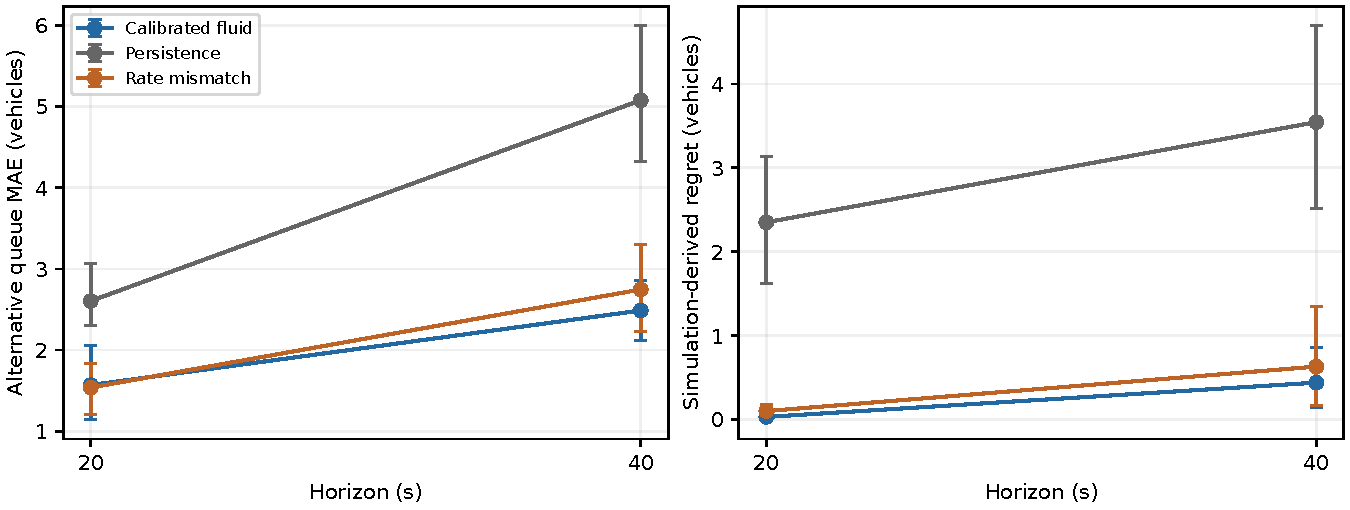
\includegraphics[width=0.96\textwidth]{figures/simulator_reference.pdf}
\caption{Alternative queue error and simulation-derived regret at the two
tested horizons. Error bars are whole-seed 95\% bootstrap percentile intervals
($n=6$); lines connect discrete conditions, not a fitted response. All demand
and policy conditions are included.}
\label{fig:sumo-reference}
\end{figure*}

\paragraph{RQ3: Trajectory preservation and execution cost}
Paired production trajectories matched in all 864 executions, and every
requested prediction completed. Mean action-commit latency was 0.050 ms for
production only, 0.568 for one shadow, 0.574 for a mirror, 0.785 for alternatives
only, 1.001 for CSC synchronous and 1.046 for CSC asynchronous execution
(Table~\ref{tab:sumo-modes}). Thus RQ3 supports trajectory preservation in this
cohort, but asynchronous execution did not reduce mean commit latency.
Mean total window wall time was 133.30 ms for production only, 138.78 ms for
synchronous and 135.64 ms for asynchronous execution. These include simulator
input/output (I/O), not isolated scheduling speedup. The evaluation process's
lifetime peak resident set size (RSS) was 43,220,992 bytes; it does not attribute
simulator memory to individual modes.

Fixed and queue-responsive policies had descriptive factual mean queues of
14.980 and 13.198 vehicles across identical anchor conditions. Their actions
were chosen without model promotion. These single-window outcomes are not
estimates of sustained closed-loop policy value.

\section{Discussion}
The architecture's measured contribution is execution and evidence admission.
Warm workers often returned complete comparisons under the tested short-run
conditions, while added delay made that evidence scarce under the configured
deadline. A controller can therefore retain production authority while losing
most of its useful alternative evidence. Production survival, completion and
durable persistence must be evaluated separately.

The mirror provides a direct model check for the action production selected.
That discrepancy arrives after the window. Using it as a prospective trust
signal would require a separate validation design; neither exact replay nor
successful isolation supplies that missing link. The evaluation preserves
incomplete and failed controls rather than treating configuration as enforcement.
The blocked continuous study and lost memory observer also prevent their
intended conclusions.

The simulator comparison evaluates a calibrated fluid predictor that uses
arrival forecasts against a stationary persistence baseline that ignores them.
It does not isolate an accuracy benefit from branching, the mirror or
asynchronous dispatch. The observed reversals under restrictions and demand
change expose the effect of omitted state and forecast assumptions. Similarly,
the absence of a mean asynchronous latency benefit in the lightweight simulator
study limits performance conclusions from logical decoupling alone.

\section{Limitations and Threats to Validity}
\paragraph{Replication and scope}
All experiments used one physical host. Logical node placement is not
independent-host fault isolation or an evaluated cloud--edge deployment.
E1 factorial cells had three run units; E2 had a single ordered resource
comparison. E3 had six seed clusters on one network, simulator version and host,
not six independent operational environments. Within-seed conditions and epochs
are correlated. With $n=6$, percentile interval reliability is limited;
the reported intervals remain descriptive and cannot support broad safety
or generalization guarantees.

\paragraph{Model and forecast validity}
The fluid anchor omits microscopic positions, travel-time pipelines and pending
insertion queues. Signal switching and discharge dynamics are simplified.
Constant past-rate forecasts cannot anticipate an unannounced change. Factual
runs and reference alternatives share SUMO dynamics and demand assumptions, so
the reference is independent of the fluid implementation but not of the
simulator environment. Replay is version/platform scoped. Turning,
pedestrians and lane changes were excluded. No predictive uncertainty model,
abstention policy or physical causal counterfactual observations exist.
Consequently, complete evidence and low simulated regret do not authorize
learning or policy promotion, which remain blocked.

\paragraph{Containment and resource limits}
The tested controls cover specified paths, not arbitrary adversarial workers,
credential theft or whole-host failure. Redis/NATS connections were authenticated
without Transport Layer Security (TLS). The single in-memory gateway has no
demonstrated durable or highly available exactly-once recovery. Memory-pressure
observer loss left its declared criterion unmet, and PID enforcement was not
exercised. CPU throttling was observed, but request-level latency samples are
not evidence of resource non-interference. Bounded records and payloads do not
prove bounded process memory. The continuous study was not executed, so
long-run memory, sustained completeness and cadence remain unresolved.
Storage faults did not cover whole-disk failure, arbitrary partial writes or
exactly-once persistence. Cadence observations are not hard-real-time guarantees.

\paragraph{Inference}
Model-based alternatives exchange statistical overlap assumptions for fidelity
and synchronization assumptions. Those assumptions are stronger than
computational replay, as counterfactual-evaluation research emphasizes
\cite{jiang2016doubly,wang2017optimal}. The policy comparison uses one decision
window rather than learned or sustained closed-loop control. Stronger
forecast-aware baselines and additional independent environments would be
needed to assess broader predictive and operational value.

\section{Conclusion}
CSC separates authoritative production from a same-action mirror and
non-actuating alternatives, with explicit evidence admission and bounded
execution. The evaluation demonstrated deterministic replay, short-run evidence
availability, selected authorization and CPU controls, and a simulator-based
comparison of forecast-only estimates with persistence. Delay collapse,
condition-specific reversals, the unexecuted continuous study and inconclusive
memory containment define the limits of those findings. Learning and policy
promotion remain blocked.

Future work should test stronger forecast-aware baselines, prospective trust
signals, sustained execution, complete resource enforcement and independent
multi-host or physical environments before operational policy use.

\section*{AI Tool Usage}
OpenAI Codex generated substantial manuscript text, the SUMO adapter,
authorization integration, experiment and analysis scripts, figures, and
publication-audit/build tools. The installed Humanize workflow supported a
focused academic editorial pass. Measurements came from the declared software
executions. Automated checks do not replace the named authors' review of
scientific claims, citations, authorship, originality or venue policy; their
approval is required before submission.

\bibliographystyle{IEEEtran}
\bibliography{references}
\end{document}
